\documentclass[conference]{IEEEtran}
\IEEEoverridecommandlockouts
% The preceding line is only needed to identify funding in the first footnote. If that is unneeded, please comment it out.
\usepackage{cite}
\usepackage{amsmath,amssymb,amsfonts}
\usepackage{algorithmic}
\usepackage[]{graphicx} % remove the draft if you need
\usepackage{textcomp}
\usepackage{xcolor}
\usepackage{booktabs}
\usepackage{subcaption}
\usepackage{url}
\usepackage[colorlinks=true, linkcolor=black, citecolor=black, urlcolor=black]{hyperref}


\usepackage{pgfplots}
\pgfplotsset{compat=1.18}
\usepackage{amsmath}

\def\BibTeX{{\rm B\kern-.05em{\sc i\kern-.025em b}\kern-.08em
    T\kern-.1667em\lower.7ex\hbox{E}\kern-.125emX}}
\begin{document}
\usepgfplotslibrary{groupplots}

\title{\LARGE
Segmentation Strategies for Long-Code Authorship Detection: Balancing Context Coverage and Computational Efficiency\\
% {\footnotesize \textsuperscript{*}Note: Sub-titles are not captured in Xplore and
% should not be used}
\thanks{Code is available at \href{https://github.com/mehedihasan88/Human-Machine-Hybrid-Adversarial-Code-Classification}{GitHub repository (https://github.com/mehedihasan88/Human-Machine-Hybrid-Adversarial-Code-Classification)}.}
}

\author{Mehedi Hasan, Mahbub Islam Mahim, Jugal Krishna Das\\
Department of Computer Science and Engineering, Jahangirnagar University, Savar, Dhaka-1342, Bangladesh\\
Correspondence E-mail: mahbubislammahim@gmail.com
}




\maketitle

\begin{abstract}
Detecting the authorship of source code becomes substantially more difficult when programs exceed the fixed context window of transformer-based models, as important stylistic and structural cues may fall outside the observed input. Although long programs are common in real-world software repositories, there is limited systematic understanding of how practical segmentation strategies influence authorship detection under such constraints. We investigate this problem by comparing three widely applicable approaches that require no modification to pretrained models: truncation-based classification, multi-view cropping with aggregation, and sliding-window classification with logit pooling. These methods reflect different trade-offs between computational cost and context coverage. All approaches are evaluated under a unified experimental setup on a length-stratified dataset that emphasizes long code samples. This study provides a controlled empirical investigation of how segmentation and aggregation choices affect accuracy, macro-F1, per-class robustness, confidence behavior, length-dependent degradation, and inference cost in long-code authorship detection. Multi-view classification substantially improves over truncation, achieving 0.896 accuracy and 0.860 macro-F1, compared to 0.862 accuracy and 0.817 macro-F1 for truncation (+3.43 and +4.31 points, respectively). Sliding-window classification attains the highest overall performance (0.897 accuracy, 0.862 macro-F1), but multi-view reaches near-parity (within 0.10 accuracy and 0.23 macro-F1) while requiring far fewer forward passes. Improvements are most pronounced for hybrid and adversarial code, where discriminative evidence is dispersed across distant regions of the program. These results indicate that context coverage is a primary factor in effective code authorship detection and provide practical guidance for selecting efficient long-context handling strategies when full-program processing is infeasible.
\end{abstract}

\vspace{0.5em}

\begin{IEEEkeywords}
code authorship detection, long-context modeling, transformer models, sliding window, multi-view aggregation, AI-generated code
\end{IEEEkeywords}

\section{Introduction}

The increasing availability of large language models (LLMs) and automated code generation systems has introduced new challenges in tracing the origin of source code. Code authorship detection has become critical for scenarios such as academic integrity enforcement in education, digital forensics in software engineering, compliance monitoring in regulated industries, and quality assurance of AI‑assisted development workflows—particularly when distinguishing between human‑written, machine‑generated, hybrid, and adversarial code. Recent benchmarks have shown that modern code generation models can produce outputs that are difficult to differentiate from human-written code, making authorship detection a challenging and evolving problem \cite{chen2021codex}\cite{fried2022incoder}.


Transformer-based models have become the dominant approach for code understanding tasks due to their ability to capture rich contextual relationships. However, these models are inherently limited by a fixed context window, restricting the length of input they can process. In real-world scenarios, source code often exceeds this limit, leading to \textit{context window overflow}, where only a portion of the code is analyzed while the rest is ignored. This is particularly problematic for authorship detection, as relevant stylistic and structural signals may be distributed across different regions of the code.

Several recent works have explored long-context modeling techniques to address this limitation. Sparse attention mechanisms such as BigBird \cite{zaheer2020bigbird} and memory-augmented transformers like Transformer-XL \cite{dai2019transformerxl} extend the effective context length by modifying the attention structure. While effective, these approaches require architectural changes and are not always directly compatible with pretrained code models. 

Alternatively, segment-based strategies have been explored, where long sequences are divided into smaller chunks and processed independently, with predictions aggregated during inference \cite{khandelwal2020generalization}. These methods offer a practical way to handle long inputs without modifying the underlying model. However, they primarily focus on model design or benchmark evaluation, and there is limited understanding of how different long-context handling strategies affect classification performance under fixed context constraints.\

This paper presents a systematic empirical study of segmentation strategies for long-code authorship detection under fixed-context transformer constraints. Unlike prior long-document classification work focused mainly on natural language, or long-context code models requiring architectural changes, our study examines practical strategies that work directly with existing pretrained code encoders. This setting is important because authorship evidence in source code may appear across initialization logic, file endings, generated blocks, hybrid regions, or adversarially modified segments.

We compare truncation, multi-view cropping, and sliding-window logit pooling using the same backbone, tokenizer, data splits, and evaluation protocol. This controlled setup isolates how context coverage and aggregation affect overall performance, per-class behavior, length-based degradation, confidence, and computational cost. The analysis offers practical guidance on when efficient multi-view cropping is sufficient and when costlier sliding-window coverage is justified.

% In this work, we address this gap by systematically comparing three practical strategies for handling long source code within fixed-context transformer models: truncation-based single-view classification, multi-view cropping with aggregation, and sliding-window classification with logit pooling. These approaches represent different trade-offs between computational efficiency and context coverage.

% We evaluate all methods under a unified experimental setup using a transformer-based classification framework and a length-stratified dataset that emphasizes long code samples. Our results show that context coverage plays a critical role in performance, with multi-view and sliding-window approaches significantly outperforming truncation, especially for challenging cases such as hybrid and adversarial code. Furthermore, multi-view achieves near-parity with sliding-window while requiring substantially lower computations, making it a strong practical choice.

\section{Related Works}

Recent advances in code authorship and AI-generated code detection have increasingly relied on transformer-based models. CodeBERT \cite{feng-etal-2020-codebert} introduces bimodal pretraining using both natural language and programming language data, enabling the model to learn joint representations of code and its textual context. It demonstrates strong performance across tasks such as code search and documentation generation. UniXcoder \cite{guo-etal-2022-unixcoder} further enhances representation learning by incorporating structural signals such as abstract syntax trees (AST) and comments. While these models provide powerful encoders, they are constrained by fixed input lengths and require additional strategies to process long source code.

Transformer-based approaches have also been applied to authorship-related tasks. CLAVE \cite{alvarezfidalgo2025clave} uses contrastive learning to distinguish whether two code samples belong to the same author. By training on large-scale datasets, it shows that transformer embeddings can capture fine-grained stylistic patterns. However, it focuses on pairwise verification rather than multi-class classification and does not address context overflow in long inputs.

Long-context handling has been widely studied in the NLP domain. Hierarchical transformers \cite{pappagari2019} process long inputs by splitting them into smaller segments, encoding each segment independently, and then aggregating segment representations through a higher-level model. Dai \textit{et al.} \cite{dai2022revisiting} demonstrate that dividing long inputs into overlapping chunks and aggregating their predictions can significantly improve performance. This approach preserves more global context compared to truncation and has been shown to improve performance on long document classification tasks. However, it introduces additional architectural complexity and requires multi-stage training.

In the context of source code, LongCoder \cite{guo2023longcoder} proposes a sparse-attention transformer for long-range code modeling. It combines sliding-window attention with global bridge tokens and memory tokens to enable information flow across distant code regions. This allows the model to capture long-range dependencies more efficiently than standard transformers. However, it requires architectural modifications and is primarily evaluated on code generation tasks rather than classification. 

Recent work such as Droid \cite{orel-etal-2025-droid} considers detection of human-written, machine-generated, hybrid, and adversarial code in a unified setting. It highlights challenges in generalization and robustness across programming languages and generation models. However, it does not systematically analyze the effect of long-context handling strategies under fixed context constraints.

In contrast, our work focuses specifically on context window overflow in transformer-based code models. We compare three practical strategies: truncation-based classification, multi-view cropping with aggregation, and sliding-window classification with logit pooling. This enables a systematic analysis of trade-offs between efficiency, context coverage, and representational fidelity in multi-class code authorship detection.

\section{Methodology}

\subsection{Problem Definition}

Code authorship detection aims to determine the origin of a given source code snippet. In this work, we formulate it as a four-class classification problem: \textit{Human}, \textit{Machine}, \textit{Hybrid}, and \textit{Adversarial}. \textit{Human} refers to code written entirely by a human developer, while \textit{Machine} represents code generated by automated systems such as large language models. \textit{Hybrid} denotes code that contains a mixture of human-written and machine-generated segments. \textit{Adversarial} includes code that has been intentionally modified to obscure its origin or to evade detection.

The task becomes challenging when dealing with long source code, as modern transformer-based models are constrained by a fixed context window. When the length of a code sample exceeds the model's maximum token limit, only a portion of the input can be processed at once. This leads to \textit{context window overflow}, where potentially informative regions of the code are excluded from analysis. Since stylistic and structural cues relevant to authorship may appear throughout the code, truncating the input can significantly degrade performance. Therefore, designing strategies to effectively utilize long code within fixed-length models is essential.

\subsection{Dataset Selection and Processing}

We conduct experiments using the SemEval-2026 Task C dataset \cite{orel-etal-2025-codet} for code authorship origin detection. The dataset consists of labeled code snippets with associated metadata, including the source code, generator information, class label, and programming language. Following the task definition, each snippet is assigned to one of four authorship-origin classes: Human, Machine, Hybrid, or Adversarial. This setting is suitable for studying long-code authorship detection because authorship-related evidence may appear in different regions of a program rather than only at the beginning of the file.

The full training file contains 900,000 labeled snippets. For the purpose of this study, we use a length-stratified training subset rather than the entire training corpus. This choice is motivated by the objective of the paper: to compare long-context handling strategies under a controlled and computationally feasible setup. In preliminary data-scaling runs, we observed that increasing the number of training snippets beyond approximately 100,000 produced only marginal performance changes. Therefore, we use a larger 200K-scale subset to retain sufficient training diversity while avoiding unnecessary computational expansion.

This design choice is especially important for the multi-view and sliding-window methods. Unlike truncation, which uses a single input sequence per snippet, multi-view cropping can create multiple views from one long snippet, and sliding-window classification can expand a single snippet into several overlapping windows. As a result, training on the full 900,000-snippet corpus would substantially increase the effective number of training instances and encoder forward passes, particularly for the sliding-window setting. The selected subset therefore provides a practical balance between dataset scale, computational cost, and fair comparison across the three segmentation strategies.

All sampling decisions are based on token length computed with the UniXcoder tokenizer, without truncation. This produces a token-length value for each snippet that matches the actual input representation used by the model. We divide snippets into short code, where the token length is at most 512, and long code, where the token length exceeds the 512-token encoder limit. The training subset is constructed with a target ratio of 20\% short snippets and 80\% long snippets so that context-window overflow remains central to the experimental setting. Long snippets are further grouped into 512-token length buckets, such as $[512,1024)$, $[1024,1536)$, and $[1536,2048)$, and samples are drawn across non-empty buckets to avoid concentrating the subset in a single length range.

The same selected training subset, tokenizer, random seed, preprocessing pipeline, validation split, and test split are used for all three methods. Therefore, any observed performance difference can be attributed to the input segmentation and aggregation strategies rather than to differences in data selection. We report the final class distributions and token-length distributions of all splits to make the effect of the length-aware sampling procedure transparent.
% All three methods operate on a subset derived from the SemEval-2026 Task C dataset, which builds upon enriched data from prior works on AI-generated code detection \cite{orel-etal-2025-codet}. The dataset contains labeled code snippets across multiple programming languages, covering diverse generators and domains, making it suitable for evaluating authorship detection under realistic conditions.

% To focus on the long-context problem, we construct a length-aware subset that includes both short and long programs, with an emphasis on longer samples. The subset is created using token length computed from the UniXcoder tokenizer, ensuring consistency with the model input representation. Rather than sampling uniformly, we adopt a length-based stratification strategy. Specifically, a smaller portion of samples is drawn from short code (token length $\leq 512$), while the majority is selected from longer code, with further stratification across multiple length ranges. This ensures coverage of both moderately long and extremely long sequences, which are critical for evaluating context window overflow.

% Validation and test sets are constructed from a separate data split and follow a similar length-aware sampling strategy. This ensures that evaluation reflects generalization to unseen data while maintaining consistency in length distribution. The same dataset construction and pre-processing pipeline is applied across all methods. This guarantees that any performance differences arise solely from the long-context handling strategies rather than variations in data sampling, enabling a fair and controlled comparison.

\subsection{Overview of Proposed Approaches}
Three distinct strategies are explored to address the context window limitation. The first approach relies on direct truncation, treating the problem as standard sequence classification within the fixed context size. The second approach introduces a multi-view representation by extracting multiple segments from different parts of the code. The third approach adopts a sliding-window mechanism that processes the entire code through overlapping segments and aggregates the results. 

These methods represent increasing levels of context preservation, ranging from minimal (truncation) to comprehensive (sliding windows). Figure~\ref{fig:3methods} provides an overview of all three methods, while Figure~\ref{fig:train} illustrates their training methodology and Figure~\ref{fig:inference} depicts the corresponding inference methodology.

\begin{figure}
    \centering
    \includegraphics[width=1\linewidth]{3.png}
    \caption{3 different methods for long sample handling}
    \label{fig:3methods}
\end{figure}

\subsection{Method 1: Truncation-Based Single-View Classification}

The first method serves as a baseline approach in which each code sample is processed as a single sequence constrained by the model's maximum token limit. When a sample exceeds this limit, it is truncated, and only the initial portion is used for classification. This approach does not attempt to recover or approximate information from the remaining parts of the program. As a result, context overflow is handled through \textit{information reduction}, where excess tokens are discarded. During both training and inference, each sample is treated as a single instance, and no additional aggregation is performed. The model directly predicts the class label based on the truncated sequence. 

While computationally efficient and straightforward, this method risks losing critical stylistic or structural signals present in later sections of the code, particularly in long or composite programs. This limitation is especially significant for hybrid authorship detection, where different segments of the same program may originate from different sources, such as a combination of human-written and machine-generated code.

\subsection{Method 2: Multi-View Cropping with Aggregation}

The second method addresses context overflow by representing each long code sample through two fixed-length views extracted from different regions of the program, specifically the beginning and the end. These regions are selected to capture complementary authorship signals, such as structural patterns at initialization and stylistic characteristics present toward the conclusion of the code. During training, each view is treated as an independent sample with the same label as the original code, effectively augmenting the dataset and enabling the model to learn from multiple parts of the program. At inference time, both views are processed separately, and their predicted logits are aggregated to produce a final prediction. The aggregation is performed using mean pooling across the two views, with an additional max-based adjustment for specific classes (e.g., adversarial) to emphasize strong localized signals.

Unlike truncation, this method performs \textit{selective context sampling}, capturing representative regions that are likely to contain distinctive authorship features. However, it still relies on a limited number of views and may miss information outside the selected segments.

\begin{figure}
    \centering
    \includegraphics[width=1\linewidth]{train.png}
    \caption{Training pipeline of the three approaches}
    \label{fig:train}
\end{figure}

\subsection{Method 3: Sliding-Window Classification with Logit Pooling}

The third method provides a more comprehensive solution by dividing long code into a sequence of overlapping segments using a sliding-window mechanism. Each segment is processed independently, and the resulting predictions are aggregated to form a final decision for the entire code sample.

A window size of $w = 512$ tokens and a stride of $s = 256$ tokens are used, producing a 50\% overlap between adjacent windows. This overlap is intentional: tokens near window boundaries appear in two consecutive segments, preventing any boundary region from being split at a disadvantageous point and ensuring that short but meaningful code constructs are always seen in full within at least one window.

During training, each window is treated as a separate training instance while preserving the original label, enabling the model to learn from all parts of the code. Because adjacent windows share 256 tokens, the same token subsequences appear in multiple training examples. Since the label is consistent across all windows of a given sample, this repeated exposure acts as implicit data augmentation on boundary-spanning patterns rather than introducing label ambiguity; no deduplication of overlapping content is required.

At inference time, all windows corresponding to a code sample are evaluated, and their logits are aggregated. The primary aggregation strategy combines mean pooling across all classes with a max-based enhancement for specific classes (e.g., adversarial), allowing the model to capture both distributed patterns and strong localized signals. Because tokens in the overlapping region contribute to two consecutive window predictions, those regions receive implicit double weighting under unweighted mean pooling. In practice this has a smoothing effect: predictions anchored to a single window boundary are averaged with the surrounding context windows, which reduces the influence of spurious signals confined to one segment edge and yields a more stable final prediction. 

In contrast to the previous methods, this approach performs \textit{full context coverage}, ensuring that the entire code is analyzed. Although more computationally intensive, it provides a more faithful representation of long code and is better suited for capturing dispersed authorship characteristics.


\begin{figure}
    \centering
    \includegraphics[width=1\linewidth]{inference.png}
    \caption{Inference-time pipeline of the three approaches}
    \label{fig:inference}
\end{figure}



\subsection{Comparative Analysis}

The three methods differ primarily in how they balance context preservation and computational efficiency. The truncation-based approach is the most efficient but discards a significant portion of long inputs, making it vulnerable to information loss. The multi-view approach improves coverage by sampling multiple regions, offering a compromise between efficiency and representational richness. The sliding-window approach provides the most complete coverage by analyzing the entire code, but at a higher computational cost. From a methodological perspective, the approaches can be seen as a progression from \textit{information reduction}, to \textit{selective sampling}, to \textit{exhaustive coverage}. This progression reflects increasing fidelity in representing long code, accompanied by increasing computational requirements.

\subsection{Implementation Details}

All methods are implemented using a transformer-based sequence classification framework with a shared architecture and training pipeline. The same model backbone, tokenizer, and optimization strategy are used across all approaches to ensure consistency. Differences arise only in how input sequences are constructed and processed before being fed into the model. No external summarization, retrieval, or prompt-based reasoning is employed. The methods rely solely on segmentation and aggregation strategies to manage long-context inputs within a fixed-size encoder.

\section{Results and Evaluation}

We present a comprehensive evaluation of the three long-context handling strategies on a held-out test set. We report overall performance metrics, per-class breakdown, length-based analysis, and confidence-based measures to provide a complete picture of each approach's strengths and limitations.

\subsection{Dataset}

We use the SemEval-2026 Task C training parquet: 900{,}000 labeled snippets with columns \texttt{code}, \texttt{generator}, \texttt{label}, and \texttt{language}. The task is four-class authorship origin detection: Human (0), Machine (1), Hybrid (2), or Adversarial (3). Rather than training on the full 900{,}000 rows, we optimize on a \textbf{length-stratified subset} (201{,}826 rows, 22.4\% of the file) to ensure long code is not drowned out by short snippets. Table~\ref{tab:train_dist} contrasts label distributions in the full corpus versus our stratified training subset. Compared with the raw data, the subset increases the Machine share (23.4\% $\rightarrow$ 28.1\%) while reducing Hybrid and Adversarial proportions. Human remains the plurality class at roughly 55\% in both distributions. This rebalancing aligns training mass more closely with the difficulty of rare or mixed-origin classes while preserving a realistic label distribution.

The most frequent languages are Python (249{,}247), Java (239{,}751), C\# (107{,}949), C++ (75{,}738), JavaScript (73{,}745), and Go (57{,}844), with the remainder spread across C, PHP, and others. Models therefore see a multi-language mix dominated by a few ecosystems; we do not stratify by language in the experiments reported here.

\begin{table}[htbp]
  \centering
  \caption{Label distribution: full training file vs.\ stratified subset used for model training (same taxonomy).}
  \label{tab:train_dist}
  \resizebox{0.9\columnwidth}{!}{%
  \begin{tabular}{@{}l rr rr@{}}
    \toprule
    & \multicolumn{2}{c}{Full file (900{,}000)} & \multicolumn{2}{c}{Training subset (201{,}826)} \\
    \cmidrule(lr){2-3} \cmidrule(lr){4-5}
    Class & Count & Share (\%) & Count & Share (\%) \\
    \midrule
    Human (0)        & 485{,}483 & 54.0 & 110{,}492 & 54.8 \\
    Machine (1)      & 210{,}471 & 23.4 &  56{,}781 & 28.1 \\
    Hybrid (2)       &  85{,}520 &  9.5 &  11{,}543 &  5.7 \\
    Adversarial (3)  & 118{,}526 & 13.2 &  23{,}010 & 11.4 \\
    \midrule
    \textbf{Total}   & 900{,}000 & 100.0 & 201{,}826 & 100.0 \\
    \bottomrule
  \end{tabular}
  }%
\end{table}

\subsection{Data Splits}

All length statistics use UniXcoder tokenizer length (\texttt{tok\_len}), matching the actual tokenization the encoder receives. The training subset (target 200{,}000, seed 42) draws 20\% of rows from $\texttt{tok\_len} \leq 512$ and 80\% from longer code, with additional allocation across long-length buckets. The realized size is 201{,}826 rows because integer bucket targets need not sum to exactly 200{,}000.

Validation and test are disjoint halves of the official Task C \emph{validation} release (33{,}743 / 33{,}742 snippets), stratified using the same short/long recipe as training. These are not random subsamples of the 900{,}000-row training parquet, so test performance reflects generalization to that independent release rather than to i.i.d.\ rows from the training file.

Table~\ref{tab:split_sizes} lists split sizes and short vs.\ long counts. Table~\ref{tab:split_labels} shows that validation and test are label-shifted relative to the training subset: Human is a smaller share ($\sim$44\%) while Hybrid and Adversarial are larger ($\sim$9.7\% / $\sim$14.4\%). This distribution shift makes the held-out split a stricter evaluation than matching the training label mix.

Table~\ref{tab:toklen_three} and Figure~\ref{fig:toklen_three} summarize tokenizer-length histograms in five bins. The training subset places more mass in the 1025+ bin than validation or test (27.3\% vs.\ $\sim$18.3\%), so models are trained on a somewhat longer-tailed length distribution than the split used for headline metrics. This design choice ensures models are exposed to challenging long-context examples during training.

\begin{table}[htbp]
  \centering
  \footnotesize
  \caption{Splits (UniXcoder \texttt{tok\_len}). Tr.\,\% = training subset as a fraction of the 900{,}000-row training release; ``---'' for val/test. Short/Long = $\leq$512 / $>$512 tokens; L\% = long share of that split.}
  \label{tab:split_sizes}
  \resizebox{0.9\columnwidth}{!}{%
  \begin{tabular}{@{}l r r r r r@{}}
    \toprule
    Split & $n$ & Tr.\,\% & $\leq$512 & $>$512 & L\% \\
    \midrule
    Training (strat.) & 201{,}826 & 22.4 & 40{,}000 & 161{,}826 & 80.2 \\
    Validation & 33{,}743 & --- & 8{,}000 & 25{,}743 & 76.3 \\
    Test & 33{,}742 & --- & 8{,}000 & 25{,}742 & 76.3 \\
    \bottomrule
  \end{tabular}
  }%
\end{table}

\begin{table}[htbp]
  \centering
  \caption{Class distribution (\%) on each split (0 Human, 1 Machine, 2 Hybrid, 3 Adversarial).}
  \label{tab:split_labels}
  \resizebox{0.9\columnwidth}{!}{%
  \begin{tabular}{@{}lcccc@{}}
    \toprule
    Split & 0 & 1 & 2 & 3 \\
    \midrule
    Training subset & 54.75 & 28.13 & 5.72 & 11.40 \\
    Validation      & 44.44 & 31.53 & 9.69 & 14.35 \\
    Test            & 44.43 & 31.53 & 9.69 & 14.35 \\
    \bottomrule
  \end{tabular}
  }%
\end{table}

\begin{table}[htbp]
  \centering
  \caption{UniXcoder \texttt{tok\_len} histogram (\% of rows in each split).}
  \label{tab:toklen_three}
  \resizebox{0.9\columnwidth}{!}{%
  \begin{tabular}{@{}lccc@{}}
    \toprule
    Bin (tokens) & Train subset & Validation & Test \\
    \midrule
    0--128     &  6.03 &  6.91 &  7.01 \\
    129--256   &  7.02 &  8.30 &  8.02 \\
    257--512   &  6.77 &  8.51 &  8.68 \\
    513--1024  & 52.92 & 57.93 & 57.98 \\
    1025+      & 27.27 & 18.37 & 18.31 \\
    \midrule
    Sum        & 100.00 & 100.00 & 100.00 \\
    \bottomrule
  \end{tabular}
  }%
\end{table}

\begin{figure}[htbp]
  \centering
  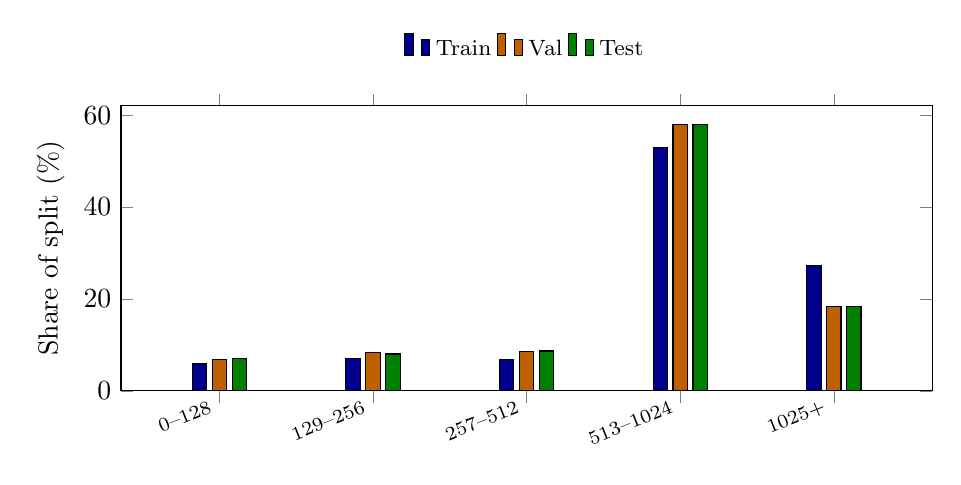
\begin{tikzpicture}
  \begin{axis}[
    width=0.98\linewidth, height=5.2cm,
    ybar,
    bar width=5.2pt,
    ymin=0, ymax=62,
    ylabel={Share of split (\%)},
    symbolic x coords={B1,B2,B3,B4,B5},
    xticklabels={0--128,129--256,257--512,513--1024,1025+},
    xtick=data,
    x tick label style={font=\scriptsize, rotate=22, anchor=east},
    enlarge x limits=0.16,
    legend style={at={(0.5,1.12)}, anchor=south, legend columns=3, draw=none, font=\footnotesize},
  ]
  \addplot[fill=blue!55!black] coordinates {(B1,6.03) (B2,7.02) (B3,6.77) (B4,52.92) (B5,27.27)};
  \addlegendentry{Train}
  \addplot[fill=orange!75!black] coordinates {(B1,6.91) (B2,8.30) (B3,8.51) (B4,57.93) (B5,18.37)};
  \addlegendentry{Val}
  \addplot[fill=green!50!black] coordinates {(B1,7.01) (B2,8.02) (B3,8.68) (B4,57.98) (B5,18.31)};
  \addlegendentry{Test}
  \end{axis}
  \end{tikzpicture}
  \caption{Tokenizer length mix for the training subset, validation, and test portions (Table~\ref{tab:toklen_three}).}
  \label{fig:toklen_three}
\end{figure}

\subsection{Experimental Setup}

We compare three strategies for fitting long code into a fixed encoder window. All runs share identical configuration: \texttt{microsoft/unixcoder-base} backbone, maximum length 512, balanced class weights, the stratified training subset described above, and \textbf{one full training epoch} with consistent optimization settings across variants. The only deliberate difference is how input sequences are cropped or tiled before the encoder.

\textbf{Truncation} keeps the head of each snippet (single forward pass per sample). \textbf{Multi-view} builds two crops (start and end) for long snippets, trains on both as separate labeled examples, and averages logits at evaluation time. \textbf{Sliding window} enumerates overlapping windows ($w{=}512$, $s{=}256$), trains on every window, and pools window logits back to a snippet prediction. This approach expands the number of gradient steps per logical snippet and, at test time, typically requires more encoder calls than multi-view (which itself uses twice as many passes as truncation on long inputs).

Headline metrics are accuracy and macro-averaged F1 on the test partition ($n{=}33{,}742$), using \texttt{true\_label}, \texttt{pred\_label}, and \texttt{tok\_len} for bucketed analysis. We also report weighted-F1, macro-averaged precision and recall, and confidence-based metrics to provide a comprehensive performance picture.

\subsection{Overall Performance}

Table~\ref{tab:main_comprehensive} reports overall performance metrics for all three methods, with 95\% bootstrap confidence intervals computed from 1,000 resamples. Truncation is clearly the weakest: multi-view achieves 0.8964 accuracy (95\% CI: [0.8931, 0.8998]) and 0.8598 macro-F1 (95\% CI: [0.8553, 0.8641]), significantly outperforming truncation which achieves 0.8621 accuracy (95\% CI: [0.8584, 0.8662]) and 0.8167 macro-F1 (95\% CI: [0.8117, 0.8217]). The non-overlapping confidence intervals indicate clear separation between truncation and multi-view, confirming that multi-view's gains of 3.43 accuracy points and 4.31 macro-F1 points are statistically significant.\\

Multi-view and sliding window achieve near-parity: sliding achieves 0.8974 accuracy (95\% CI: [0.8940, 0.9006]) and 0.8621 macro-F1 (95\% CI: [0.8574, 0.8666]). The small differences of 0.10 accuracy points and 0.23 macro-F1 points fall within overlapping confidence intervals, indicating that these differences are within statistical noise rather than representing a meaningful performance gap. Macro-F1 is the stricter headline metric because it weights the four classes equally and is sensitive to Hybrid and Adversarial errors under the label shift in Table~\ref{tab:split_labels}.

Table~\ref{tab:main_comprehensive} also reveals that weighted-F1 closely tracks accuracy across all methods, reflecting Human's dominance as the plurality class. Macro-precision and macro-recall follow similar patterns, with multi-view and sliding showing balanced improvements over truncation.

\begin{table}[htbp]
  \centering
  \caption{Comprehensive performance metrics on the held-out test set ($n{=}33{,}742$). One training epoch per model.}
  \label{tab:main_comprehensive}
  \footnotesize
  \setlength{\tabcolsep}{2.5pt}
  \resizebox{0.9\columnwidth}{!}{%
  \begin{tabular}{@{}lccccc@{}}
    \toprule
    Method & Acc. & Macro-F1 & Wgt.-F1 & Prec. & Rec. \\
    \midrule
    Trunc. & 0.8621 & 0.8167 & 0.8632 & 0.8131 & 0.8209 \\
    Multi-view & 0.8964 & 0.8598 & 0.8976 & 0.8511 & 0.8698 \\
    Sliding & \textbf{0.8974} & \textbf{0.8621} & 0.8982 & \textbf{0.8577} & 0.8676 \\
    \bottomrule
  \end{tabular}
  }%
\end{table}



\subsection{Per-Class Analysis}

Table~\ref{tab:perclass} breaks down F1 scores by class, with 95\% bootstrap confidence intervals reported in the main comprehensive metrics table. Human and Machine are the easiest categories under all three methods, with F1 in the 0.85--0.96 range. This reflects their relatively consistent stylistic patterns compared to mixed-origin code.

Hybrid remains the most challenging class: truncation reaches only 0.7137 F1 (95\% CI: [0.7013, 0.7260]), while multi-view and sliding improve this to 0.7836 (95\% CI: [0.7734, 0.7941]) and 0.7985 (95\% CI: [0.7876, 0.8097]) respectively---a gain of roughly seven to eight and a half absolute points. The confidence intervals confirm that these improvements are statistically significant.

To illustrate why Hybrid is challenging, consider a concrete failure case: a Hybrid snippet of 1,072 tokens (test index 24306) contains Human-written code in the head but Machine-generated code at the tail. Truncation, which only processes the first 512 tokens, predicts this sample as Machine with 0.89 confidence, missing the Machine characteristics beyond its window. Multi-view and sliding window, which also process the tail of the file, correctly identify this as Hybrid. This example demonstrates how Hybrid snippets with asymmetric code distributions are particularly vulnerable to truncation errors, explaining why multi-view and sliding reduce Hybrid$\rightarrow$Machine confusion from 34\% (truncation) to 21--20\% (multi-view/sliding).

Adversarial F1 improves from 0.7663 (95\% CI: [0.7572, 0.7749]) with truncation to 0.8127 (95\% CI: [0.8042, 0.8201]) / 0.8075 (95\% CI: [0.7986, 0.8156]) with multi-view / sliding. Notably, multi-view slightly outperforms sliding on Adversarial (0.8127 vs.\ 0.8075), demonstrating that the expensive tiling strategy does not uniformly beat the two-crop design on every class.

These patterns align with the semantic positioning of each class: Hybrid snippets occupy a narrow band between Human and Machine origins, making them particularly sensitive to how evidence is aggregated across different code regions. The consistent advantage of multi-view and sliding over truncation on Hybrid and Adversarial suggests that capturing evidence from multiple code regions is crucial for distinguishing mixed-origin code.

\begin{table}[htbp]
  \centering
  \caption{Per-class F1 scores on the held-out test split.}
  \label{tab:perclass}
  \resizebox{0.9\columnwidth}{!}{%
  \begin{tabular}{@{}lcccc@{}}
    \toprule
    Method & Human & Machine & Hybrid & Adv. \\
    \midrule
    Truncation   & 0.9356 & 0.8513 & 0.7137 & 0.7663 \\
    Multi-view   & 0.9610 & 0.8818 & 0.7836 & 0.8127 \\
    Sliding win. & 0.9613 & 0.8812 & 0.7985 & 0.8075 \\
    \bottomrule
  \end{tabular}
  }%
\end{table}

Figure~\ref{fig:cm_comparison} visualizes confusion matrices, revealing error patterns. Hybrid samples show the highest confusion with both Human and Machine classes. Truncation (Figure~\ref{fig:cm_trunc}) exhibits the most confusion. Hybrid samples are frequently misclassified as Machine (34\%, 663 samples) and Human (14\%, 114 samples). Misclassified Hybrid samples have mean confidence of 0.67 (median: 0.65), with only 11.5\% high-confidence ($\geq$0.9). In contrast, correctly classified Hybrid samples have mean confidence of 0.84 (median: 0.89) and 47.1\% high-confidence. Multi-view (Figure~\ref{fig:cm_multi}) substantially reduces confusion. Hybrid$\rightarrow$Machine drops to 21\% (433 samples) and Hybrid$\rightarrow$Human to 16\% (66 samples). Misclassified Hybrid confidence rises to 0.76, while correct Hybrid reaches 0.91 with 71.3\% high-confidence. Sliding window (Figure~\ref{fig:cm_slide}) achieves similar improvements. Hybrid$\rightarrow$Machine is at 20\% (520 samples) and Hybrid$\rightarrow$Human at 19\% (63 samples). The confidence gap between correct (0.91) and incorrect (0.75) Hybrid samples remains, indicating Hybrid remains the most challenging class.

\begin{figure*}[htbp]
  \centering
  \begin{subfigure}{0.32\textwidth}
    \centering
    \includegraphics[width=\linewidth]{confusion_matrix_truncation.png}
    \caption{Truncation}
    \label{fig:cm_trunc}
  \end{subfigure}
  \hfill
  \begin{subfigure}{0.32\textwidth}
    \centering
    \includegraphics[width=\linewidth]{confusion_matrix_multiview.png}
    \caption{Multi-view}
    \label{fig:cm_multi}
  \end{subfigure}
  \hfill
  \begin{subfigure}{0.32\textwidth}
    \centering
    \includegraphics[width=\linewidth]{confusion_matrix_sliding.png}
    \caption{Sliding Window}
    \label{fig:cm_slide}
  \end{subfigure}
  \caption{Confusion matrices for the three methods on the test set. Each $4 \times 4$ matrix shows normalized proportions (color intensity) with raw counts in parentheses. Diagonal cells indicate correct predictions, while off-diagonal cells show confusion patterns.}
  \label{fig:cm_comparison}
\end{figure*}

\subsection{Performance by Length Buckets}

To understand where long-context modeling helps, we bucket test examples by \texttt{tok\_len} and recompute macro-F1 within each bucket (Table~\ref{tab:buckets} and Figure~\ref{fig:buckets}). Performance degrades monotonically as snippets grow: all methods lose ground past $\sim$1k tokens, and the longest bucket ($\geq 2560$) is far below the short-code bins. This trend confirms the intuition that authorship labels depend on evidence distributed across the file, which becomes harder to aggregate as windows multiply.

Multi-view improves macro-F1 over truncation in \emph{every} bucket, confirming that the second crop is never harmful in aggregate. Sliding and multi-view are close overall but show complementary strengths: multi-view is slightly ahead in the $\leq 512$ and $[1024,1536)$ bins, while sliding leads in the dense middle bin $[512,1024)$ and on the extreme tail $\geq 2560$. Neither method uniformly wins across all buckets, reinforcing the interpretation that they represent different operating points on a cost--accuracy curve rather than a strict performance ordering.

The dramatic drop in performance for the longest bucket (Macro-F1 $\sim$0.32--0.41) highlights a fundamental challenge: even with sliding-window coverage, aggregating evidence across extremely long sequences remains difficult. This suggests opportunities for more sophisticated long-context strategies, such as hierarchical attention or learned importance weighting.

\begin{table}[htbp]
  \centering
  \caption{Macro-F1 by tokenizer length bucket (held-out test, same $n$ per row).}
  \label{tab:buckets}
  \resizebox{0.9\columnwidth}{!}{%
  \begin{tabular}{@{}lccc@{}}
    \toprule
    Bucket & Trunc. & Multi-v. & Sliding \\
    \midrule
    $\leq 512$      & 0.7956 & 0.8237 & 0.8217 \\
    $[512,1024)$    & 0.7718 & 0.8421 & \textbf{0.8530} \\
    $[1024,1536)$   & 0.6716 & \textbf{0.7175} & 0.7139 \\
    $[1536,2048)$   & 0.6670 & \textbf{0.7001} & 0.6981 \\
    $[2048,2560)$   & 0.4447 & 0.4727 & 0.4809 \\
    $\geq 2560$     & 0.3166 & 0.3463 & \textbf{0.4145} \\
    \bottomrule
  \end{tabular}
  }%
\end{table}

\begin{figure}[htbp]
  \centering
  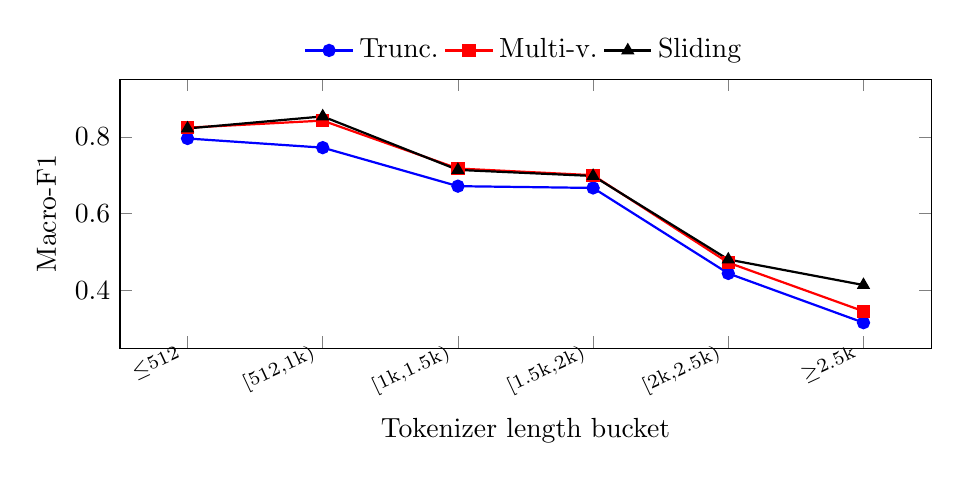
\begin{tikzpicture}
  \begin{axis}[
    width=0.98\linewidth, height=5cm,
    ylabel={Macro-F1},
    xlabel={Tokenizer length bucket},
    xmin=0.5, xmax=6.5,
    ymin=0.25, ymax=0.95,
    xtick={1,2,3,4,5,6},
    xticklabels={%
      {$\leq$512},%
      {[512,1k)},%
      {[1k,1.5k)},%
      {[1.5k,2k)},%
      {[2k,2.5k)},%
      {$\geq$2.5k}%
    },
    x tick label style={font=\scriptsize, rotate=25, anchor=east},
    legend style={at={(0.5,1.02)}, anchor=south, legend columns=3, draw=none},
  ]
  \addplot[thick, mark=*, blue] coordinates {(1,0.7956) (2,0.7718) (3,0.6716) (4,0.6670) (5,0.4447) (6,0.3166)};
  \addlegendentry{Trunc.}
  \addplot[thick, mark=square*, red] coordinates {(1,0.8237) (2,0.8421) (3,0.7175) (4,0.7001) (5,0.4727) (6,0.3463)};
  \addlegendentry{Multi-v.}
  \addplot[thick, mark=triangle*, black] coordinates {(1,0.8217) (2,0.8530) (3,0.7139) (4,0.6981) (5,0.4809) (6,0.4145)};
  \addlegendentry{Sliding}
  \end{axis}
  \end{tikzpicture}
  \caption{Macro-F1 vs.\ length bucket (Table~\ref{tab:buckets}). Performance degrades monotonically with code length, but multi-view and sliding consistently outperform truncation.}
  \label{fig:buckets}
\end{figure}

\subsection{Confidence Analysis}

Model confidence provides additional insight into prediction reliability and offers practical guidance for deployment. Table~\ref{tab:confidence} summarizes confidence statistics, computed from the maximum class probability (\texttt{max\_prob}).

\begin{table}[htbp]
  \centering
  \caption{Confidence analysis on the held-out test set.}
  \label{tab:confidence}
  \footnotesize
  \setlength{\tabcolsep}{2pt}
  \resizebox{0.9\columnwidth}{!}{%
  \begin{tabular}{@{}lccc@{}}
    \toprule
    Method & Conf. (Corr.) & Conf. (Incorr.) & High Conf. ($\geq$0.9) \\
    \midrule
    Trunc. & 0.9019 & 0.6461 & 62.3\% (0.9784) \\
    Multi-view & 0.9484 & 0.7219 & 77.6\% (0.9729) \\
    Sliding & 0.9504 & 0.7353 & 78.8\% (0.9691) \\
    \bottomrule
  \end{tabular}
  }%
\end{table}

Confidence is a reliable signal of prediction accuracy. All methods show a substantial gap between mean confidence for correct vs.\ incorrect predictions (0.22--0.26 points). Multi-view and sliding achieve higher overall confidence (0.9484/0.9504 vs.\ 0.9019) with larger high-confidence fractions (77.6\%/78.8\% vs.\ 62.3\%).

\textbf{Practical deployment trade-offs:} At a 0.9 threshold, multi-view covers 77.6\% of samples with 97.3\% accuracy. Raising to 0.95 covers 71\% at 98.3\% accuracy, flagging only 29\% for human review. Truncation requires a lower threshold (0.8) for similar coverage (73\%), with lower accuracy (95.8\%). This demonstrates that multi-view and sliding enable higher accuracy at any coverage level, making them suitable for practical systems with limited review capacity.

\subsection{Computational Considerations}

The three methods represent distinct computational trade-offs. We quantify the total forward passes required on the test set (33,742 samples, 76.3\% exceeding 512 tokens).

\textbf{Truncation} requires exactly one forward pass per sample at both training and inference time: 33,742 total passes (1.00 passes/sample). This is the most computationally efficient approach, but the efficiency comes at the cost of discarding potentially critical information in long code.

\textbf{Multi-view} requires two forward passes for samples longer than 512 tokens (start and end crops), and one pass for shorter samples. On the test set: short samples ($8{,}000 \leq 512$) require 8,000 passes, and long samples ($25{,}742 > 512$) require 51,484 passes, totaling 59,484 forward passes (1.76 passes/sample). This represents a 76.3\% overhead over truncation. During training, this effectively doubles the dataset size for long samples, increasing gradient steps and wall-clock time proportionally.

\textbf{Sliding window} requires $N = \lceil (L - w) / s \rceil + 1$ forward passes for a sample of length $L$ with window size $w{=}512$ and stride $s{=}256$. The average number of passes for long samples is 3.16, resulting in 89,222 total forward passes on the test set (2.64 passes/sample). This represents a 164.4\% overhead over truncation and a 50.0\% overhead over multi-view. For the longest bucket ($\geq$2560 tokens), samples require 8+ forward passes each, making inference 3--5$\times$ slower than multi-view for very long code.

Given the minimal performance gap between multi-view and sliding (0.10 accuracy, 0.23 macro-F1), multi-view offers a compelling efficiency--accuracy trade-off for many applications: it captures most of the accuracy benefit of comprehensive context coverage with roughly half the computational cost of sliding window for long code. Sliding window may be justified when maximum accuracy is critical and computational resources are abundant, or when processing exceptionally long sequences where the 2-crop design is insufficient.

\subsection{Discussion}

\textbf{Key findings:} Context coverage matters substantially. Multi-view and sliding window outperform truncation by large margins (3.43 accuracy points, 4.31 macro-F1 points), demonstrating that even a second crop captures critical information. Benefits concentrate on challenging cases: Hybrid F1 improves most with extra views, and the longest snippets remain difficult despite comprehensive coverage. This suggests that while simple context multiplication helps, evidence aggregation strategies become critical as sequences grow.

Methods have complementary strengths. Multi-view leads on Adversarial, suggesting adversarial signals are more localized. Sliding excels on the longest buckets, while multi-view leads on mid-length ranges. They represent different operating points on a cost--accuracy curve, not a strict ordering.

\textbf{Practical recommendations:} Model calibration improves with context coverage. Multi-view and sliding produce higher-confidence predictions with larger high-confidence fractions than truncation, making them suitable for systems that need to identify uncertain predictions for human review. Multi-view offers the best efficiency--accuracy balance for most applications, capturing most benefits with half the computational cost of sliding window for long code. Sliding window is justified when maximum accuracy is critical or for exceptionally long sequences.

\subsection{Takeaway Summary}

Multi-view and sliding window significantly outperform truncation (3.43 accuracy points, 4.31 macro-F1 points) by capturing evidence from multiple code regions. These gains are statistically significant and concentrated on challenging Hybrid samples and long code. Multi-view offers the best efficiency--accuracy balance for most applications, while sliding window is justified for maximum accuracy needs. Confidence thresholds enable practical human-in-the-loop deployment, with multi-view achieving 98.3\% accuracy on 71\% of samples.

\subsection{Limitations and Future Work}

This study has a few limitations that suggest directions for future research:

\textbf{No language stratification.} The dataset mixes multiple programming languages without language-specific modeling. Authorship signals may vary by language, and context coverage requirements could differ across languages (e.g., verbose Java vs.\ concise Python).

\textbf{Extreme long-context challenge.} The $\geq$2560 bucket shows that even sliding window struggles with extremely long code. Hierarchical transformers, sparse attention mechanisms, or retrieval-based approaches may be needed to effectively model these cases.

\textbf{Limited fine-grained error analysis.} While we analyze confusion patterns and confidence-conditioned errors, we have not examined specific code features or patterns that lead to misclassifications. Fine-grained error analysis could reveal insights into authorship signals and guide method improvements.

\section{Conclusions}
We evaluated three long-context handling strategies for code authorship detection. Context coverage substantially impacts performance: moving from truncation to multi-view improves accuracy by 3.43 points (0.8621 to 0.8964) and macro-F1 by 4.31 points (0.8167 to 0.8598), demonstrating that even a second crop captures critical information.

Multi-view and sliding window achieve near-parity (0.10 accuracy, 0.23 macro-F1 gaps), suggesting diminishing returns beyond two crops. Benefits concentrate on challenging cases: Hybrid F1 improves most (0.7137 to 0.7985), while the longest snippets remain difficult ($\geq$2560 bucket: macro-F1 0.32--0.41). Simple context multiplication helps but is insufficient for extreme long-context---evidence aggregation becomes critical. Multi-view offers an excellent efficiency--accuracy trade-off, capturing most coverage benefits with roughly half the computational cost of sliding window. We recommend multi-view for most applications, with sliding window justified when maximum accuracy is critical or for exceptionally long code. Confidence thresholds can effectively identify uncertain predictions for human review.

Future work should explore language-specific modeling, hierarchical attention for extreme long-context, and systematic error pattern analysis. This work demonstrates the importance of long-context handling and provides practical guidance for method selection.

\section*{Acknowledgment}
The authors used AI-assisted writing tools to improve the clarity and readability of the manuscript text. All scientific content, experimental design, data analysis, and conclusions are solely the work of the authors.

% Trigger a column break in the bibliography at reference N so that
% all three biographies land together on the final page(s).
% Adjust the number (try 4, 5, 6 ...) until all bios stay together.
\IEEEtriggeratref{5}
\bibliographystyle{IEEEtran}
\bibliography{references}

\begin{IEEEbiography}[{\includegraphics[width=1in,height=1.25in,clip,keepaspectratio]{Mahim.jpg}}]{Mahbub Islam Mahim}
received the B.Sc. and M.Sc. degrees in Computer Science and Engineering from Jahangirnagar University, Dhaka, Bangladesh, in 2021 and 2023, respectively. During his master's studies, he was awarded the National Science and Technology Fellowship by the Ministry of Science and Technology, Bangladesh. He is currently a Senior Software Engineer at the Samsung R\&D Institute Bangladesh. His work includes knowledge graph technologies, generative AI, semantic reasoning systems, and full-stack development. He has also contributed to patent development, including an A1-graded patent in 2025. Mahim's research interests include trustworthy AI, knowledge representation, and advanced machine learning applications. He has authored publications in NLP, generative AI, and computer vision, including a best-paper award--winning work on Bangla hate speech detection at AACL-IJCNLP 2025. He has also received multiple awards and recognitions for innovation and technical excellence at Samsung.
\end{IEEEbiography}

\begin{IEEEbiography}[{\includegraphics[width=1in,height=1.25in,clip,keepaspectratio]{mehedi.jpeg}}]{Mehedi Hasan}
is a software engineer and researcher with expertise in artificial intelligence and wearable systems. He works at Samsung R\&D Institute Bangladesh, where he contributes to agentic systems, natural language processing, and the development of Galaxy Watch projects. His work includes developing an interactive prior-art search and multi-stage obviousness-detection agent for patent analysis, designing machine-learning solutions to estimate liquid consumption using wearable devices, and contributing to Android and WearOS system development for Samsung wearables. Alongside his industry role, Mehedi is active in academic research, focusing on AI for software engineering, image processing, and low-resource language technologies. His contributions include an award-winning framework for Bangla hate speech detection, with academic and professional awards recognizing his success and commitment to developing practical, reliable, and human-centered AI solutions.
\end{IEEEbiography}

\begin{IEEEbiography}[{\includegraphics[width=1in,height=1.25in,clip,keepaspectratio]{Jugal_sir.jpg}}]{Dr. Jugal Krishna Das}
has completed his B.Sc., M.Sc., and Ph.D. degrees in Computer Engineering from Donetsk Technical University, Ukraine. He is currently a Professor in the Department of Computer Science and Engineering at Jahangirnagar University, Savar, Dhaka, Bangladesh. Dr. Das's research interests include Computer Networks, Machine Learning, Natural Language Processing, and Software Engineering. His key fields of interest encompass System Design and Analysis, E-commerce, Management Information Systems, Database Management Systems, Computer Architecture, Data Structures and Algorithms, Microprocessors, Computer Networking, Discrete Mathematics, Digital Logic Design, Operating Systems, Parallel and Distributed Systems, Internet Engineering, and IP Technology. He has 48 publications in Computer Science and Engineering in national and international journals and conference proceedings.
\end{IEEEbiography}

\end{document}
